\documentclass[10pt]{article}
\usepackage[polish]{babel}
\usepackage[utf8]{inputenc}
\usepackage[T1]{fontenc}
\usepackage{amsmath}
\usepackage{amsfonts}
\usepackage{amssymb}
\usepackage[version=4]{mhchem}
\usepackage{stmaryrd}
\usepackage{graphicx}
\usepackage[export]{adjustbox}
\graphicspath{ {./images/} }
\usepackage{multirow}

\title{\begin{tabular}{|c|}
\(\begin{array}{c}\text { Miejsce } \\ \text { na naklejkę }\end{array}\) \\
EGZAMIN MATURALNY \\
\end{tabular} Z MATEMATYKI \\
 POZIOM PODSTAWOWY }

\author{}
\date{}


\begin{document}
\maketitle
\section*{Czas pracy 120 minut}
\section*{Instrukcja dla zdającego}
\begin{enumerate}
  \item Sprawdź, czy arkusz egzaminacyjny zawiera 19 stron (zadania 1-12). Ewentualny brak zgłoś przewodniczącemu zespołu nadzorującego egzamin.
  \item Rozwiązania zadań i odpowiedzi zamieść w miejscu na to przeznaczonym.
  \item W rozwiązaniach zadań przedstaw tok rozumowania prowadzacy do ostatecznego wyniku.
  \item Pisz czytelnie. Używaj długopisu/pióra tylko z czarnym tuszem/atramentem.
  \item Nie używaj korektora, a błędne zapisy przekreśl.
  \item Pamiętaj, że zapisy w brudnopisie nie podlegają ocenie.
  \item Obok każdego zadania podana jest maksymalna liczba punktów, którą możesz uzyskać za jego poprawne rozwiązanie.
  \item Możesz korzystać z zestawu wzorów matematycznych, cyrkla i linijki oraz kalkulatora.
  \item Na karcie odpowiedzi wpisz swoją datę urodzenia i PESEL. Nie wpisuj żadnych znaków w części przeznaczonej dla egzaminatora.
\end{enumerate}

MAJ\\
ROK 2008\\

\includegraphics[max width=\textwidth, center]{2024_11_21_2f72fc0c2faed8928619g-01(1)}

Za rozwiązanie wszystkich zadań można otrzymać łącznie 50 punktów

\section*{Życzymy powodzenia!}
Wypehnia zdający\\
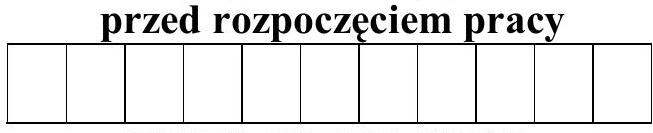
\includegraphics[max width=\textwidth, center]{2024_11_21_2f72fc0c2faed8928619g-01}

PESEL ZDAJĄCEGO\\
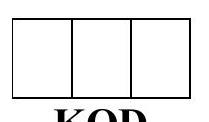
\includegraphics[max width=\textwidth, center]{2024_11_21_2f72fc0c2faed8928619g-01(2)}

KOD\\
ZDAJĄCEGO

\section*{Zadanie 1. (4 pkt)}
Na poniższym rysunku przedstawiono łamaną \(A B C D\), która jest wykresem funkcji \(y=f(x)\).\\
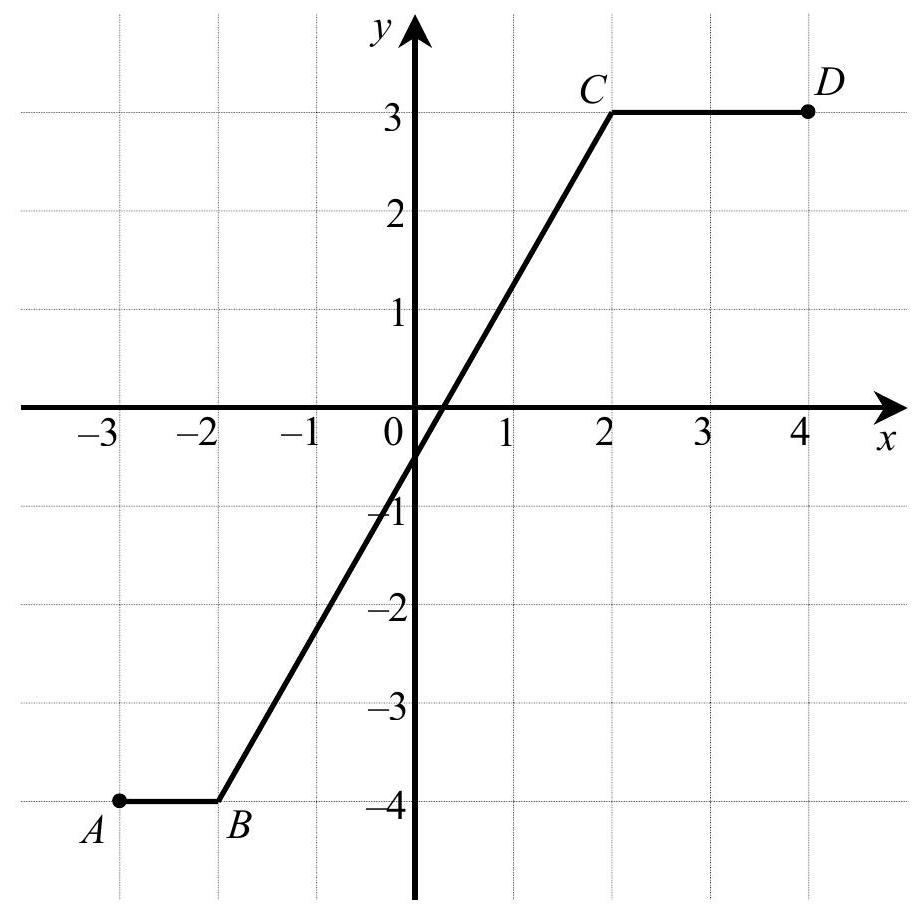
\includegraphics[max width=\textwidth, center]{2024_11_21_2f72fc0c2faed8928619g-02}

Korzystajac z tego wykresu:\\
a) zapisz w postaci przedziału zbiór wartości funkcji \(f\),\\
b) podaj wartość funkcji \(f\) dla argumentu \(x=1-\sqrt{10}\),\\
c) wyznacz równanie prostej \(B C\),\\
d) oblicz długość odcinka \(B C\).\\

\includegraphics[max width=\textwidth, center]{2024_11_21_2f72fc0c2faed8928619g-02(1)}\\

\includegraphics[max width=\textwidth, center]{2024_11_21_2f72fc0c2faed8928619g-03}

\begin{center}
\begin{tabular}{|c|l|c|c|c|c|}
\hline
\multirow{2}{*}{\begin{tabular}{c}
Wypetnia \\
egzaminator! \\
\end{tabular}} & Nr zadania & 1.1 & 1.2 & 1.3 & 1.4 \\
\cline { 2 - 6 }
 & Maks. liczba pkt & 1 & 1 & 1 & 1 \\
\cline { 2 - 6 }
 & Uzyskana liczba pkt &  &  &  &  \\
\hline
\end{tabular}
\end{center}

\section*{Zadanie 2. (4 pkt)}
Liczba przekątnych wielokąta wypukłego, w którym jest \(n\) boków i \(n \geq 3\) wyraża się wzorem \(P(n)=\frac{n(n-3)}{2}\).\\
Wykorzystując ten wzór:\\
a) oblicz liczbę przekątnych w dwudziestokacie wypukłym.\\
b) oblicz, ile boków ma wielokąt wypukły, w którym liczba przekątnych jest pięć razy większa od liczby boków.\\
c) sprawdź, czy jest prawdziwe następujące stwierdzenie:

Każdy wielokat wypukly o parzystej liczbie boków ma parzystq liczbę przekatnych. Odpowiedź uzasadnij.\\

\includegraphics[max width=\textwidth, center]{2024_11_21_2f72fc0c2faed8928619g-04}

\begin{center}
\begin{tabular}{|c|l|c|c|c|c|}
\hline
\multirow{2}{*}{\begin{tabular}{c}
Wypelnia \\
egzaminator! \\
\end{tabular}} & Nr zadania & 2.1 & 2.2 & 2.3 & 2.4 \\
\cline{2-6} & Maks. liczba pkt & 1 & 1 & 1 & 1 \\
\cline{2-6} & Uzyskana liczba pkt &  &  &  &  \\
\hline
\end{tabular}
\end{center}

\section*{Zadanie 3. (4 pkt)}
Rozwią̇̇ równanie \(4^{23} x-32^{9} x=16^{4} \cdot\left(4^{4}\right)^{4}\).\\
Zapisz rozwiązanie tego równania w postaci \(2^{k}\), gdzie \(k\) jest liczbą całkowitą.\\

\includegraphics[max width=\textwidth, center]{2024_11_21_2f72fc0c2faed8928619g-05}

\begin{center}
\begin{tabular}{|c|l|c|c|c|c|}
\hline
\multirow{2}{*}{\begin{tabular}{c}
Wypelnia \\
egzaminator! \\
\end{tabular}} & Nr zadania & 3.1 & 3.2 & 3.3 & 3.4 \\
\cline { 2 - 6 }
 & Maks. liczba pkt & 1 & 1 & 1 & 1 \\
\cline { 2 - 6 }
 & Uzyskana liczba pkt &  &  &  &  \\
\hline
\end{tabular}
\end{center}

\section*{Zadanie 4. (3 pkt)}
Koncern paliwowy podnosił dwukrotnie w jednym tygodniu cenę benzyny, pierwszy raz o \(10 \%\), a drugi raz o \(5 \%\). Po obu tych podwyżkach jeden litr benzyny, wyprodukowanej przez ten koncern, kosztuje 4,62 zł. Oblicz cenę jednego litra benzyny przed omawianymi podwyżkami.\\

\includegraphics[max width=\textwidth, center]{2024_11_21_2f72fc0c2faed8928619g-06}

\begin{center}
\begin{tabular}{|c|l|c|c|c|}
\hline
\multirow{2}{*}{\begin{tabular}{c}
Wypetnia \\
egzaminator! \\
\end{tabular}} & Nr zadania & 4.1 & 4.2 & 4.3 \\
\cline { 2 - 5 }
 & Maks. liczba pkt & 1 & 1 & 1 \\
\cline { 2 - 5 }
 & Uzyskana liczba pkt &  &  &  \\
\hline
\end{tabular}
\end{center}

\section*{Zadanie 5. (5 pkt)}
Nieskończony ciąg liczbowy \(\left(a_{n}\right)\) jest określony wzorem \(a_{n}=2-\frac{1}{n}, n=1,2,3, \ldots\).\\
a) Oblicz, ile wyrazów ciągu \(\left(a_{n}\right)\) jest mniejszych od \(1,975\).\\
b) Dla pewnej liczby \(x\) trzywyrazowy ciag \(\left(a_{2}, a_{7}, x\right)\) jest arytmetyczny. Oblicz \(x\).\\

\includegraphics[max width=\textwidth, center]{2024_11_21_2f72fc0c2faed8928619g-07}

\begin{center}
\begin{tabular}{|c|l|c|c|c|c|c|}
\hline
\multirow{2}{*}{\begin{tabular}{c}
Wypelnia \\
egzaminator! \\
\end{tabular}} & Nr zadania & 5.1 & 5.2 & 5.3 & 5.4 & 5.5 \\
\cline { 2 - 7 }
 & Maks. liczba pkt & 1 & 1 & 1 & 1 & 1 \\
\cline { 2 - 7 }
 & Uzyskana liczba pkt &  &  &  &  &  \\
\hline
\end{tabular}
\end{center}

\section*{Zadanie 6. (5 pkt)}
Prosta o równaniu \(5 x+4 y-10=0\) przecina oś \(O x\) układu współrzędnych w punkcie \(A\) oraz oś \(O y\) w punkcie \(B\). Oblicz współrzędne wszystkich punktów \(C\) leżących na osi \(O x\) i takich, że trójkąt \(A B C\) ma pole równe 35 .\\

\includegraphics[max width=\textwidth, center]{2024_11_21_2f72fc0c2faed8928619g-08}\\

\includegraphics[max width=\textwidth, center]{2024_11_21_2f72fc0c2faed8928619g-09}

\begin{center}
\begin{tabular}{|c|l|c|c|c|c|c|}
\hline
\multirow{2}{*}{\begin{tabular}{c}
Wypełnia \\
egzaminator! \\
\end{tabular}} & Nr zadania & 6.1 & 6.2 & 6.3 & 6.4 & 6.5 \\
\cline { 2 - 7 }
 & Maks. liczba pkt & 1 & 1 & 1 & 1 & 1 \\
\cline { 2 - 7 }
 & Uzyskana liczba pkt &  &  &  &  &  \\
\hline
\end{tabular}
\end{center}

\section*{Zadanie 7. (4 pkt)}
Dany jest trapez, w którym podstawy mają długość 4 cm i 10 cm oraz ramiona tworzą z dłuższą podstawą kąty o miarach \(30^{\circ}\) i \(45^{\circ}\). Oblicz wysokość tego trapezu.\\

\includegraphics[max width=\textwidth, center]{2024_11_21_2f72fc0c2faed8928619g-10}\\

\includegraphics[max width=\textwidth, center]{2024_11_21_2f72fc0c2faed8928619g-11}

\begin{center}
\begin{tabular}{|c|l|c|c|c|c|}
\hline
\multirow{2}{*}{\begin{tabular}{c}
Wypełnia \\
egzaminator! \\
\end{tabular}} & Nr zadania & 7.1 & 7.2 & 7.3 & 7.4 \\
\cline { 2 - 6 }
 & Maks. liczba pkt & 1 & 1 & 1 & 1 \\
\cline { 2 - 6 }
 & Uzyskana liczba pkt &  &  &  &  \\
\hline
\end{tabular}
\end{center}

\section*{Zadanie 8. (4 pkt)}
Dany jest wielomian \(W(x)=x^{3}-5 x^{2}-9 x+45\).\\
a) Sprawdź, czy punkt \(A=(1,30)\) należy do wykresu tego wielomianu.\\
b) Zapisz wielomian \(W\) w postaci iloczynu trzech wielomianów stopnia pierwszego.\\

\includegraphics[max width=\textwidth, center]{2024_11_21_2f72fc0c2faed8928619g-12}

\begin{center}
\begin{tabular}{|c|l|c|c|c|c|}
\hline
\multirow{2}{*}{\begin{tabular}{c}
Wypelnia \\
egzaminator! \\
\end{tabular}} & Nr zadania & 8.1 & 8.2 & 8.3 & 8.4 \\
\cline { 2 - 6 }
 & Maks. liczba pkt & 1 & 1 & 1 & 1 \\
\hline
 & Uzyskana liczba pkt &  &  &  &  \\
\hline
\end{tabular}
\end{center}

Zadanie 9. (5 pkt)\\
Oblicz najmniejszą i największą wartość funkcji kwadratowej \(f(x)=(2 x+1)(x-2)\) w przedziale \(\langle-2,2\rangle\).\\

\includegraphics[max width=\textwidth, center]{2024_11_21_2f72fc0c2faed8928619g-13}

\begin{center}
\begin{tabular}{|c|l|c|c|c|c|c|}
\hline
\multirow{2}{*}{\begin{tabular}{c}
Wypełnia \\
egzaminator! \\
\end{tabular}} & Nr zadania & 9.1 & 9.2 & 9.3 & 9.4 & 9.5 \\
\cline { 2 - 7 }
 & Maks. liczba pkt & 1 & 1 & 1 & 1 & 1 \\
\hline
 & Uzyskana liczba pkt &  &  &  &  &  \\
\hline
\end{tabular}
\end{center}

\section*{Zadanie 10. (3 pkt)}
Rysunek przedstawia fragment wykresu funkcji \(h\), określonej wzorem \(h(x)=\frac{a}{x}\) dla \(x \neq 0\).\\
Wiadomo, że do wykresu funkcji \(h\) należy punkt \(P=(2,5)\).\\
a) Oblicz wartość współczynnika \(a\).\\
b) Ustal, czy liczba \(h(\pi)-h(-\pi)\) jest dodatnia czy ujemna.\\
c) Rozwią̇̇ nierówność \(h(x)>5\).\\
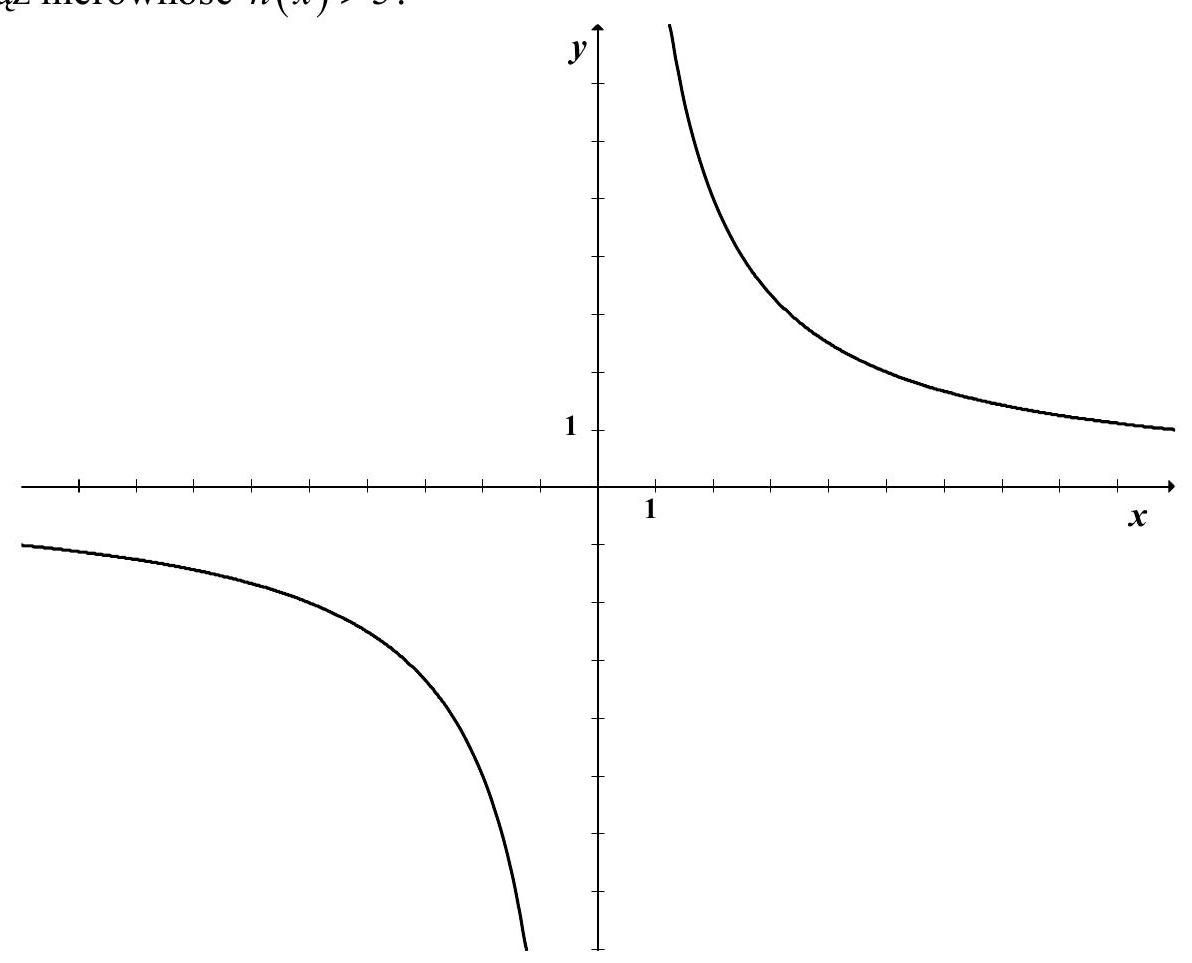
\includegraphics[max width=\textwidth, center]{2024_11_21_2f72fc0c2faed8928619g-14}\\

\includegraphics[max width=\textwidth, center]{2024_11_21_2f72fc0c2faed8928619g-14(1)}\\

\includegraphics[max width=\textwidth, center]{2024_11_21_2f72fc0c2faed8928619g-15}

\section*{Zadanie 11. (5 pkt)}
Pole powierzchni bocznej ostrosłupa prawidłowego trójkątnego równa się \(\frac{a^{2} \sqrt{15}}{4}\), gdzie a oznacza długość krawędzi podstawy tego ostrosłupa. Zaznacz na poniższym rysunku kąt nachylenia ściany bocznej ostrosłupa do płaszczyzny jego podstawy. Miarę tego kąta oznacz symbolem \(\beta\). Oblicz \(\cos \beta\) i korzystajac z tablic funkcji trygonometrycznych odczytaj przybliżoną wartość \(\beta\) z dokładnością do \(1^{\circ}\).\\
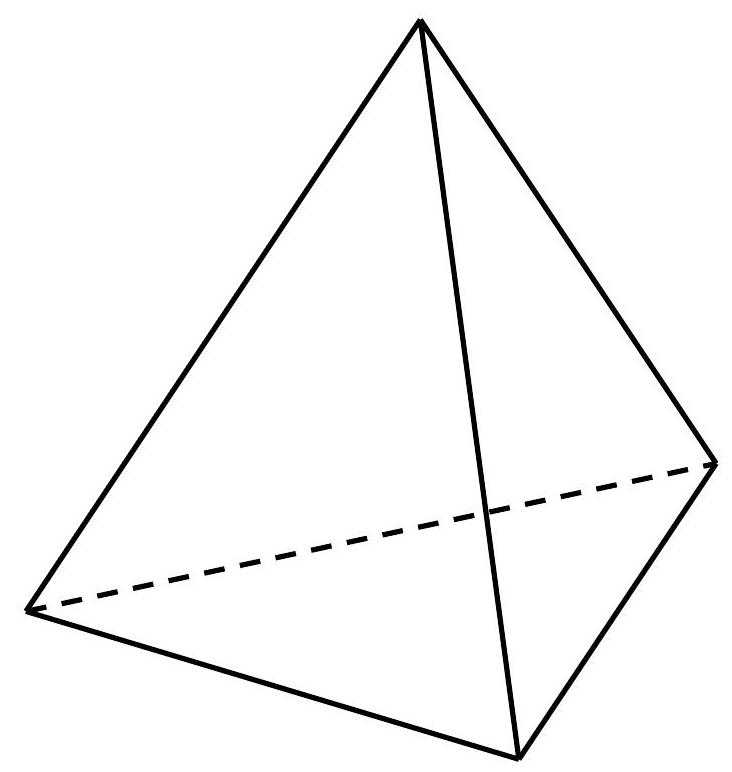
\includegraphics[max width=\textwidth, center]{2024_11_21_2f72fc0c2faed8928619g-16(5)}

\begin{center}
\begin{tabular}{|c|c|c|c|c|c|c|c|c|c|c|c|c|c|c|c|c|c|c|c|c|c|c|c|c|c|c|c|c|c|}
\hline
 &  &  &  &  &  &  &  &  &  &  &  &  &  &  &  &  &  &  &  &  &  &  &  &  &  &  &  &  &  \\
\hline
 &  &  &  &  &  &  &  &  &  &  &  &  &  &  &  &  &  &  &  &  &  &  &  &  &  &  &  &  &  \\
\hline
 &  &  &  &  &  &  &  &  &  &  &  &  &  &  &  &  &  &  &  &  &  &  &  &  &  &  &  &  &  \\
\hline
 &  &  &  &  &  &  &  &  &  &  &  &  &  &  &  &  &  &  &  &  &  &  &  &  &  &  &  &  &  \\
\hline
 &  &  &  &  &  &  &  &  &  &  &  &  &  &  &  &  &  &  &  &  &  &  &  &  &  &  &  &  &  \\
\hline
 &  &  &  &  &  &  &  &  &  &  &  &  &  &  &  &  &  &  &  &  &  &  &  &  &  &  &  &  &  \\
\hline
 &  &  &  &  &  &  &  &  &  &  &  &  &  &  &  &  &  &  &  &  &  &  &  &  &  &  &  &  &  \\
\hline
 &  &  &  &  &  &  &  &  &  &  &  &  &  &  &  &  &  &  &  &  &  &  &  &  &  &  &  &  &  \\
\hline
 &  &  &  &  &  &  &  &  &  &  &  &  &  &  &  &  &  &  &  &  &  &  &  &  &  &  &  &  &  \\
\hline
 &  &  &  &  &  &  &  &  &  &  &  &  &  &  &  &  &  &  &  &  &  &  &  &  &  &  &  &  &  \\
\hline
 &  &  &  &  &  &  &  &  &  &  &  &  &  &  &  &  &  &  &  &  &  &  &  &  &  &  &  &  &  \\
\hline
 &  &  &  &  &  &  &  &  &  &  &  &  &  &  &  &  &  &  &  &  &  &  &  &  &  &  &  &  &  \\
\hline
 &  &  &  &  &  &  &  &  &  &  &  &  &  &  &  &  &  &  &  &  &  &  &  &  &  &  &  &  &  \\
\hline
 &  &  &  &  &  &  &  &  &  &  &  &  &  &  &  &  &  &  &  &  &  &  &  &  &  &  & 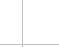
\includegraphics[max width=\textwidth]{2024_11_21_2f72fc0c2faed8928619g-16}
 &  &  \\
\hline
 &  &  &  &  &  &  &  &  &  &  &  &  &  &  &  &  &  &  &  &  &  &  &  &  &  &  &  &  &  \\
\hline
 &  &  &  &  &  &  &  &  &  &  &  &  &  &  &  &  &  &  &  &  &  &  &  &  &  &  &  &  &  \\
\hline
 &  &  &  &  &  &  &  &  &  &  &  &  &  &  &  &  &  &  &  &  &  &  &  &  &  &  &  &  &  \\
\hline
 &  &  &  &  &  &  &  &  &  &  &  &  &  &  &  &  &  &  &  &  &  &  &  &  &  &  &  &  &  \\
\hline
 &  &  &  &  &  &  &  &  &  &  &  &  &  &  &  &  &  &  &  &  &  &  &  & 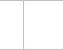
\includegraphics[max width=\textwidth]{2024_11_21_2f72fc0c2faed8928619g-16(2)}
 &  &  & 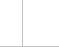
\includegraphics[max width=\textwidth]{2024_11_21_2f72fc0c2faed8928619g-16(1)}
 &  &  \\
\hline
 &  &  &  &  &  &  &  &  &  &  &  &  &  &  &  &  &  &  &  &  &  &  &  &  &  &  &  &  &  \\
\hline
 &  &  &  &  &  &  &  &  &  &  &  &  &  &  &  &  &  &  &  &  &  &  &  & \( 7 \) &  &  & 
\includegraphics[max width=\textwidth]{2024_11_21_2f72fc0c2faed8928619g-16(3)}
 &  &  \\
\hline
 &  &  &  &  &  &  &  &  &  &  &  &  &  &  &  &  &  &  &  &  &  &  &  & 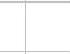
\includegraphics[max width=\textwidth]{2024_11_21_2f72fc0c2faed8928619g-16(4)}
 &  &  &  &  &  \\
\hline
 &  &  &  &  &  &  &  &  &  &  &  &  &  &  &  &  &  &  &  &  &  &  &  & - &  &  & - &  &  \\
\hline
 &  &  &  &  &  &  &  &  &  &  &  &  &  &  &  &  &  &  &  &  &  &  &  &  &  &  &  &  &  \\
\hline
\end{tabular}
\end{center}

\begin{center}

\includegraphics[max width=\textwidth]{2024_11_21_2f72fc0c2faed8928619g-17}
\end{center}

\begin{center}
\begin{tabular}{|c|l|c|c|c|c|c|}
\hline
\multirow{2}{*}{\begin{tabular}{c}
Wypetnia \\
egzaminator! \\
\end{tabular}} & Nr zadania & 11.1 & 11.2 & 11.3 & 11.4 & 11.5 \\
\cline { 2 - 7 }
 & Maks. liczba pkt & 1 & 1 & 1 & 1 & 1 \\
\hline
 & Uzyskana liczba pkt &  &  &  &  &  \\
\hline
\end{tabular}
\end{center}

\section*{Zadanie 12. (4 pkt)}
Rzucamy dwa razy symetryczną sześcienną kostką do gry. Oblicz prawdopodobieństwo każdego z następujących zdarzeń:\\
a) \(A-w\) każdym rzucie wypadnie nieparzysta liczba oczek.\\
b) \(B\) - suma oczek otrzymanych w obu rzutach jest liczbą większą od 9 .\\
c) \(C\) - suma oczek otrzymanych w obu rzutach jest liczbą nieparzystą i większą od 9 .\\

\includegraphics[max width=\textwidth, center]{2024_11_21_2f72fc0c2faed8928619g-18}

\begin{center}
\begin{tabular}{|c|l|c|c|c|c|}
\hline
\multirow{2}{*}{\begin{tabular}{c}
Wypełnia \\
egzaminator! \\
\end{tabular}} & Nr zadania & 12.1 & 12.2 & 12.3 & 12.4 \\
\cline { 2 - 6 }
 & Maks. liczba pkt & 1 & 1 & 1 & 1 \\
\cline { 2 - 6 }
 & Uzyskana liczba pkt &  &  &  &  \\
\hline
\end{tabular}
\end{center}

\section*{BRUDNOPIS}

\end{document}